\documentclass[a4paper,preprint]{sig-alternate}

\usepackage{times}
\usepackage{helvet}
\usepackage{courier}
\usepackage{microtype}
\usepackage{hyperref}
\usepackage{csquotes}

\frenchspacing

\toappear{}

\usepackage{blindtext}

\begin{document}

\title{Robustness \& Graph (Convolutional) Neural Networks}

\subtitle{Machine Learning Seminar 20/21}

\numberofauthors{1}
%
\author{
%
\alignauthor Tim Bohne\\
\email{tbohne@uni-osnabrueck.de}
}

\maketitle

\begin{abstract}
    \begin{quote}
    Graph neural networks enable the use of machine learning approaches for graph structured data.
    However, the models have proven to be prone to adversarial attacks, which questions their use in practical applications
    and leads to an increased focus on methods to strengthen their robustness. The intent of this paper is to provide a concise overview
    of the current state of research in the domain of graph (convolutional) neural networks with a focus on the robustness of these models. 
    \end{quote}
\end{abstract}

\section{Introduction}

One of the most successful types of models in the field of deep learning is the convolutional neural network (CNN).
Hence, the idea is to generalize CNNs, which are designed to operate on Euclidean data with a spatial relation like 
images and text, to graph structured data. \cite{Liu_2020}
The notion of graph embeddings, which learn to represent graph structures as low-dimensional vectors, provides
another motivation for graph neural networks. \cite{Liu_2020}
Liu et al. also highlight that traditional machine learning methods for graph analysis involve a lot of manual feature engineering
which causes them to be rather inflexible and expensive.
These considerations, along with the performance of GNNs in practical applications mentioned in section \ref{sec:background}, 
indicate that the study of GNNs and their robustness is worthwhile.
In the following sections, a concise overview of the current state of robustness focused research in the domain of GNNs is provided.\newline

After presenting some background for graph neural networks (GNNs) and particularly graph convolutional networks (GCNs)
and their possible practical applications as well as the idea of robustness in general in section \ref{sec:background}, 
an overview of the current state of the literature is provided in section \ref{sec:literature}. Subsequently, the core ideas,
methods, and results of the first works on certifiable robustness of GNNs are introduced in section \ref{sec:main_section}.
Finally, there is a conclusion and a brief outlook on possible future research in section \ref{sec:conclusion}.

\section{Background}
\label{sec:background}

A currently very active research area inside the field of machine learning, or more precisely deep learning, considers models to learn
from graph inputs. Those models are called graph neural networks (GNNs). 
Many real-life applications can be represented by a graph as data structure, e.g. \textit{"modeling physical systems, learning molecular fingerprints,
controlling traffic networks, and recommending friends in social networks"} \cite{Liu_2020}. 
Therefore, it is reasonable to think about combining graphs as data structures with state-of-the-art machine learning models.
Unfortunately, in its non-Euclidean nature, graph data is not suitable for traditional deep learning models that are typically designed 
to work with Euclidean data such as images in computer vision or text in natural language processing. \cite{Liu_2020}
There are numerous reports of convincing performance of GNNs in practical applications (e.g. \cite{NIPS2015_f9be311e},
\cite{hamilton2018inductive}, \cite{trivedi2017knowevolve}), especially in the task of semi-supervised node classification. \cite{xu2019topology}
Further typical applications for graphs as non-Euclidean data structure in machine learning are link prediction and clustering. \cite{Zhou_2019}
In summary, GNNs are models to conduct deep learning with graph data.\newline

\subsection{Graph Neural Networks}

In this section, the basic graph neural network model proposed by Scarselli et al. \cite{Scarselli_2009} gets introduced
based on the description in \textit{'Introduction to graph neural networks'}\cite{Liu_2020}.
A GNN's goal is to learn a state embedding $h_v \in \mathbb{R}^S$ for each node $v$ to generate an output $o_v$.
As an example for such an output, they name the distribution of the predicted node label.
In the original GNN model, which works with an undirected homogeneous graph, each node $v$ has input features $x_v$
as well as a set of edges $co[v]$ and neighbors $ne[v]$. 
The authors illustrate the structure with the example in fig. \ref{fig:graph}
where $x_{1}$ is the input feature of $l_1$, $co[l_1]$ contains the edges $\{l_{(1, 2)}, l_{(1, 4)}, l_{(1, 6)}, l_{(3, 1)}\}$, and 
$ne[l_1]$ contains the nodes $\{l_2, l_3, l_4, l_6\}$.

\begin{figure}[h]
    \centering
    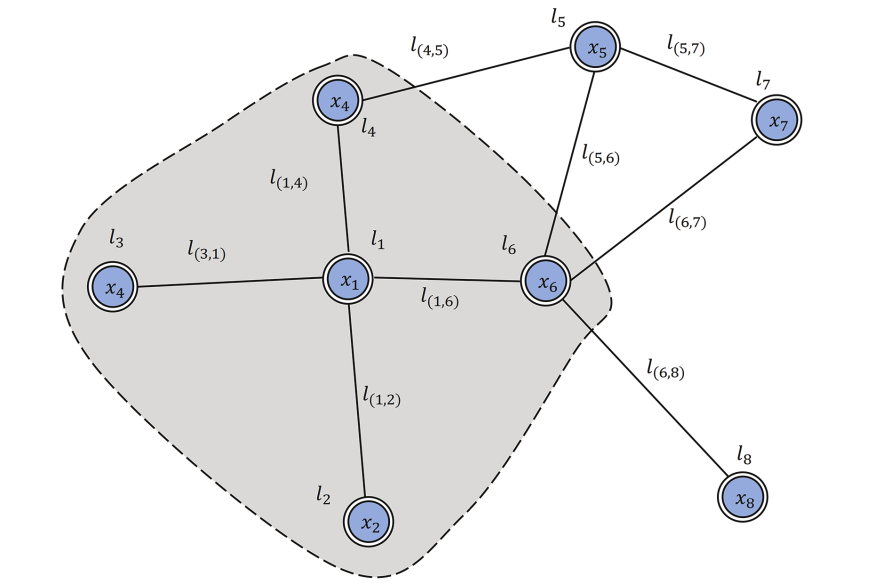
\includegraphics[width=0.4\textwidth]{img/graph.png}
    \caption{Example of the graph based on Scarselli et al. \cite{Liu_2020}}
    \label{fig:graph}
\end{figure}

There are two important functions, $f$ updates the node state based on the input neighborhood and $g$ computes the output of a node.
Let $x$ be the input feature and $h$ the hidden state:
\begin{itemize}
    \item \textbf{node embedding:} $h_v = f(x_v, x_{co[v]}, h_{ne[v]}, x_{ne[v]})$
    \item \textbf{output embedding:} $o_v = g(h_v, x_v)$
\end{itemize}

Therefore, $f$ takes as input the features of the node ($x_v$), the features of its edges ($x_{co[v]}$), the states ($h_{ne[v]}$),
and the features of the nodes in its neighborhood ($x_{ne[v]}$). The node embedding $h_v$ is then used in $g$ to compute the output of $v$.
Usually, $h_v$ and $o_v$ are described in a more compact form as matrices of stacked states $H$,
outputs $O$, and features $X$ (and node features $X_N$) with $F$ and $G$ being the stacked versions of $f$ and $g$:

\begin{itemize}
    \item $H = F(H, X)$
    \item $O = G(H, X_N)$
\end{itemize}

The $(t + 1)$-th iteration of $H$ is described as $H^{t + 1} = F(H^t, X)$.
Using the target information $t_v$ for node $v$ and the number of supervised nodes $p$, 
the loss term is described as $\sum_{i=1}^p (t_i - o_i)$ and a gradient-descent algorithm is proposed as learning technique.\newline

\vfill
\pagebreak

This basic GNN model is still rather limited, but nevertheless an important milestone on the way to making
neural networks applicable in the graph domain. \cite{Liu_2020}
The restrictions give rise to numerous flavors of GNNs, such as graph convolutional networks (GCNs),
which address certain limitations of the basic model.\newline

\textbf{Graph Convolutional Networks}\newline

The properties that define the different variants of GNNs are typically the aggregator that gathers 
information about the neighborhood of a node and a particular updater to update the hidden states. \cite{Zhou_2019}
In general, there is a certain functional evaluation of a node's features together with the features of its neighbors (convolution). 
The results are then the input for the neural network. GCN models are usually classified as spectral or spatial approaches.
Spectral approaches perform an eigendecomposition of the graph Laplacian and operate on spectral graph representations. \cite{Zhou_2019}
Whereas spatial methods work directly on the graph structure and consider the local neighborhood of nodes \cite{Zhou_2019},
which lets them appear as the more intuitive approaches.
A simple schematic representation of a deep GCN is depicted in fig. \ref{fig:gcn} where we have an initial graph as input
that is sequentially processed through the hidden layers and finally results in an output representation of the graph.
\begin{figure}[h]
    \centering
    \includegraphics[width=0.45\textwidth]{img/gcn.png}
    \caption{Multi-layer GCN. \cite{Kipf_2016}}
    \label{fig:gcn}
\end{figure}

\subsection{Robustness}

Besides the repeatedly demonstrated good performance, there is one major issue that is subject to a rather new branch of 
research inside the field of GNNs, which is the robustness of such models. There are several publications that analyze 
the robustness of GNNs to adversarial examples and recently there came up first approaches to strengthen
or even to certify their robustness with regard to a certain perturbation set.\newline
Graph neural networks have lately reached state-of-the-art performance in recommendation systems. \cite{Ying_2018}
Ying et al. developed a large-scale recommendation engine and deployed it at a major tech company.
This example illustrates the need for robust GNNs. Although these systems may be relatively rare in practical applications, especially at
that scale, at the moment, their performance suggests that this will change soon. However, in order to be able to use such models
with a clear conscience in practical applications requires a certain degree of robustness.
At the moment, there are noteworthy concerns about the security of using GNNs in safety-critical applications as they are
vulnerable to adversarial attacks. \cite{Jin_2020_Graph}\newline

\textbf{Adversarial Perturbations}\newline

A well-studied problem of machine learning models in general is their sensitivity to adversarial perturbations. \cite{Goodfellow_2015}
The idea of such perturbations, which is visualized in fig. \ref{fig:adversarial_example}, is that slight changes to the input data
cause an entirely different output of the model and therefore often misclassification.

\begin{figure}[h]
    \centering
    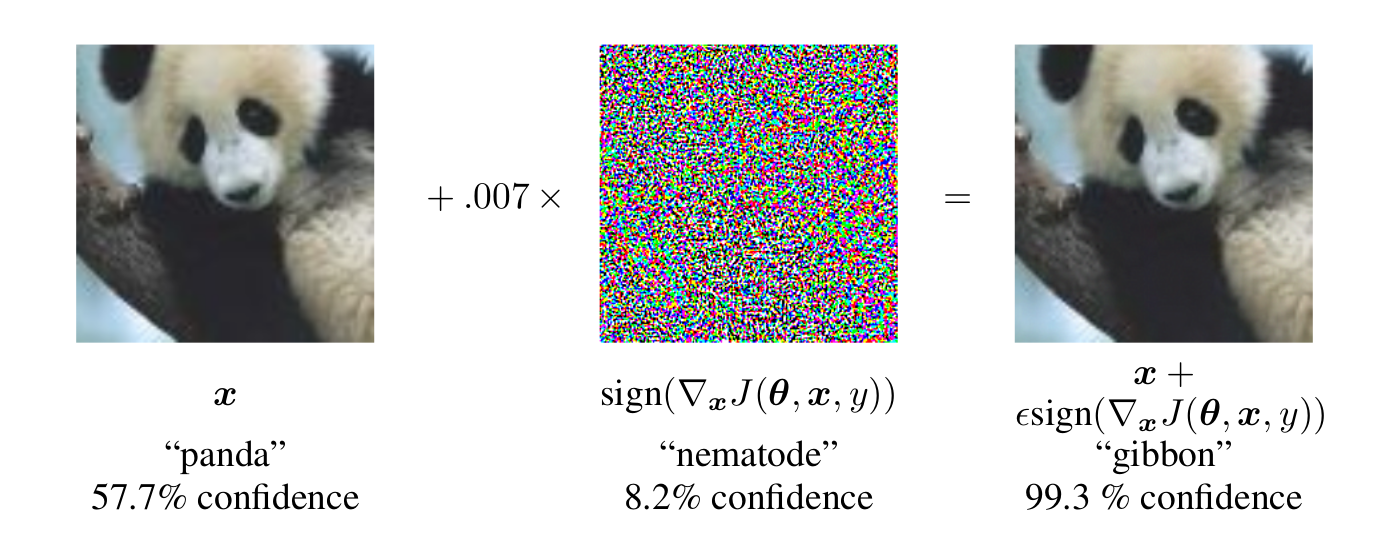
\includegraphics[width=0.5\textwidth]{img/adversarial_example.png}
    \caption{Demonstration of a fast adversarial example. \cite{Goodfellow_2015}}
    \label{fig:adversarial_example}
\end{figure}

Goodfellow et al. \cite{Goodfellow_2015} face that problem by adversarial training, which means that they include adversarially 
perturbed examples into the training process in order to strengthen the robustness of the models. Furthermore, they introduce 
efficient ways of generating adversarial examples, as shown in fig. \ref{fig:adversarial_example}.
Although the added vector in fig. \ref{fig:adversarial_example} is imperceptibly small, it suffices to change the classification
of the image by the well-known GoogleNet. \cite{Goodfellow_2015}\newline
Adversarial perturbations are not only a problem for classical machine learning models, but also for GNNs.
Numerous publications confirm the non-robustness of graph neural networks by showing that the models are prone to
adversarial attacks on the node attributes as well as on the graph structure. \cite{Zuegner_2019}
Similarly to the example in fig. \ref{fig:adversarial_example}, small perturbations to the graph structure or node features 
cause a misclassification of the target node as depicted in fig. \ref{fig:adversarial_GNN}.

\begin{figure}[h]
    \centering
    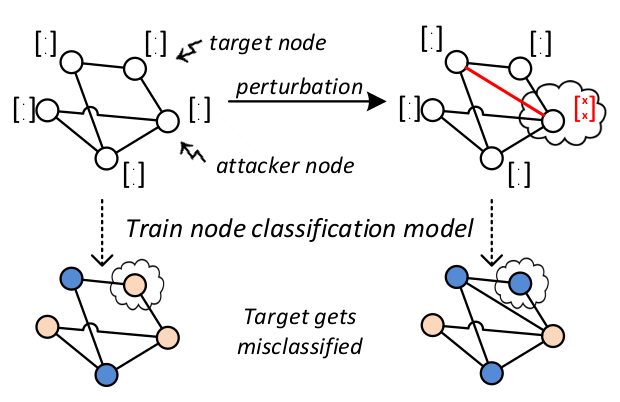
\includegraphics[width=0.35\textwidth]{img/adversarial_GNN.png}
    \caption{Small perturbations of the graph structure or node attributes cause a misclassification of the target. \cite{Zuegner_2018}}
    \label{fig:adversarial_GNN}
\end{figure}

\section{Literature Review}
\label{sec:literature}

This section will provide an overview of the current state of research in the domain of robust GNNs, which could be divided
roughly into three important phases.
The first phase was to show that GNNs are indeed vulnerable to adversarial perturbations of the graph structure and the node attributes (cf. \ref{sec:rev1}).
Afterwards, in the second phase, several publications introduced defense mechanisms against such attacks or novel training procedures 
to strengthen the robustness of the models in some scenarios (cf. \ref{sec:rev2}). Only recently, the third phase began, in which first approaches appeared
that are able to not only provide mitigations to adversarial attacks in some scenarios, but to give provable guarantees about the (non-)robustness 
of a model, which is crucial to use them in safety-critical applications in the real world (cf. \ref{sec:rev3}). Because of the relevance of the last phase, 
which is an important step in the process of bringing the convincingly performing GNN models into the real world, the main focus of the following sections
will be on publications from that phase.

\vfill
\pagebreak

\subsection{Vulnerability of GNNs to adversarial perturbations}
\label{sec:rev1}

Dai et al. \cite{Dai_2018} address adversarial attacks on graph structured data, in which the combinatorial structure of 
the data is altered in order to manipulate the outcome. They are able to show the vulnerability of GNN models to these kind of attacks
in graph-level as well as node-level classification tasks using real-world and artificial data.\newline
Another approach for adversarial attacks on graph structured data is proposed by Zügner et al. \cite{Zuegner_2018} who focus on node classification
via graph convolutional networks. The authors claim that specifically areas in which GNNs are applied, such as websites, are often target of
adversarial attacks and that it is therefore important to investigate the robustness of such models. They study adversarial attacks on attributed graphs 
and distinguish between adversarial attacks on the node's features and the graph structure.
The results suggest that even slight perturbations significantly deteriorate the classification accuracy, which clearly motivates reflections
on the robustness of such models, especially when considering practical applications.\newline
So far, adversarial attacks were introduced as a quite vague concept. Zügner et al. \cite{zuegner2019adversarial}
define them as \textquote{small deliberate perturbations of data samples in order to achieve the outcome desired by the attacker}
and propose different categories to be considered in the attack model. Furthermore, they confirm previous claims that 
even slight perturbations of the graph structure or the node attributes consistently decrease the performance of GCN models.

\subsection{Defense mechanisms}
\label{sec:rev2}

Since the fact that GNNs are vulnerable to adversarial perturbations was confirmed by many publications, the next natural question to ask
is how to defend them against such attacks.
The defense mechanisms based on adversarial samples for classical neural networks are not directly and especially not efficiently
extensible to GCNs. \cite{Jin_2020} Jin et al. tackle the problem and try to increase the efficiency by perturbations of the hidden representations
of GCNs, which means that there is no need to generate adversarial networks and therefore improved efficiency. Additionally, they state that
their framework improves robustness and accuracy in experiments on several tasks such as node classification, link prediction, and recommendation
systems.
When considering the robustness of GNNs, it is of course quite important to have efficient and effective attack methods to test with.
Xu et al. \cite{xu2019topology} are proposing an effective gradient-based attack for graph neural networks that causes decreased classification
performance. As a training procedure for higher robustnesss, they introduce an optimization-based adversarial training that is not
impairing the classification accuracy.
Zhu et al. \cite{10.1145/3292500.3330851} develop an approach that they refer to as \textit{Robust GCN} (RGCN), which is aiming at
increased robustness against adversarial attacks. To be able to simply absorb the effects of adversarial perturbations, they model
the latent structures in each layer of the GCN as being Gaussian distributed with the idea that the perturbations perish in the variances
of the distributions. According to these variances, the neighborhoods of nodes are assigned different weights to prevent adversarial attacks
from being propagated through the net. The presented experimental evaluation suggests that the goal of increased robustness is achieved.
Another approach to enhance the robustness of GCNs is proposed by Chen et al. \cite{Chen_2020} and relies on the idea that a crucial 
aspect of adversarial attacks on graph structures is given by manipulations of the edges of the graph.
Thus, they focus on mitigating the sensitivity of the models to such manipulations by a training procedure, in which
random, sparse and deformed subgraphs are used by a removal of certain edges. Experimentally, they can show that the method is indeed
mitigating the sensitivity to adversarial attacks and thereby increasing the robustness.
The idea, the approach of Jin et al \cite{Jin_2020_Graph} is based on, is that a reasonable defense method against graph perturbations lets
the perturbed version of the graph undergo some kind of cleaning procedure. The authors state that graph structures representing problems
from the real-world often share some intrinsic properties such as low-rankedness, sparsity, and a certain similarity between neighboring
nodes and that those features can be used to identify adversarial attacks, which seem to be likely to violate such properties.
Based on that idea, they propose the framework \textit{Pro-GNN}, which leads to a robust GNN model with remarkable performance in experiments
with real-world data and extensive perturbations.
Finally, Wang et al. \cite{Wang_2019} present with \textit{GraphDefense} an algorithm to improve the robustness of graph convolutional 
networks against adversarial attacks with a particular focus on scaling for large graph inputs. 
Moreover, crucial characteristics of defense methods in general are discussed to improve the robustness.

\subsection{Certifiable Robustness}
\label{sec:rev3}

When considering safety-critical applications, it is not only required to be able to defend the system in some scenarios, but there
have to be guarantees about the security of the system.
Bojchevski et al. \cite{bojchevski2019certifiable} introduce a first method that is able to verify certifiable robustness or
non-robustness of a general class of models including GNNs against perturbations of the graph structure.
An important aspect of approaches that aim to make GNNs more robust is that they should not compromise the predictive accuracy of the models.
The authors satisfy this constraint with their training process that leads to a larger fraction of nodes that are provably robust
and is even able to improve the predictive accuracy in some cases.
However, the approaches are restricted in the sense that they are not applicable to GCNs, but only to a certain class of models
based on \textit{PageRank}. \cite{10.1145/3394486.3403217}
Zügner et al. \cite{Zuegner_2019} develop a first method that deals with certifiable (non-)robustness of GCNs against perturbations
of the node attributes. The robustness certificates are always given under the assumption of a certain attack model and do not hold in general.
Hence, a node that is certified as being robust by their method is guaranteed to be robust under every possible perturbation that is part of the
defined attack model. Analogously, they are able to provide non-robustness certificates.
Adhering to the aforementioned requirement of not, or at least only minimally affecting the predictive accuracy,
the authors present a robust, semi-supervised training method.
Recently, Zügner et al. \cite{10.1145/3394486.3403217} tackle the related problem of GCNs against perturbation of the graph structure
and introduce a method for certifying their robustness. The authors reformulate the problem in a way that enables them to use specially 
optimized LP-solvers such as CPLEX to solve it. To achieve that, they express the problem as a jointly-constrained bilinear program, 
develop a branch-and-bound procedure to obtain lower bounds on the optimal solution value and are able to divide the problem into linear 
sub-problems.
Finally, Wang et al.\cite{Wang_2020} extend the so-called \textit{randomized smoothing} technique to provide robustness guarantees for any
GNN for node classification as well as graph classification problems. As Zügner et al. \cite{10.1145/3394486.3403217}, they consider
perturbations of the graph structure.

\section{Certifiable robustness of graph neural networks}
\label{sec:main_section}

As seen in the previous sections, graph neural networks are not at all robust against adversarial perturbations of the graph
structure or the node attributes. This section will provide an overview of the crucial and only recently started 
third phase of research in the domain of robust GNNs, which aims to give provable guarantees about the (non-)robustness of a model.
Only such guarantees enable the use of GNNs in safety-critical real-world applications.\newline
A first work on certifiable (non-)robustness of GNNs against perturbations of the graph structure
is proposed by Bojchevski et al. \cite{bojchevski2019certifiable}. They are able to compute certificates very efficiently
and, as mentioned in the previous section, develop a training method that leads to a higher number of nodes that are provably robust without
negatively affecting the prediction accuracy. However, due to the restriction to a class of models
based on \textit{PageRank} \cite{10.1145/3394486.3403217}, the approach will not be further discussed in this work.\newline 
After a somewhat deeper consideration of the approaches of Zügner et al., providing first robustness certificates for GCNs with respect to 
perturbations of the node attributes in section \ref{sec:paper_two} and the graph structure in section \ref{sec:paper_three},
a brief overview of the latest work on certifiable robustness of GNNs against adversarial structural perturbations is provided 
in section \ref{sec:paper_four}.

\subsection{Robustness Certification for Node Attribute Perturbations}
\label{sec:paper_two}

In this section, the approach of Zügner et al. \cite{Zuegner_2019} will be described,
in which the authors develop a first method that deals with certifiable (non-)robustness of GCNs against perturbations of
the node attributes. Since the robustness certificates are always given under the assumption of a certain attack model,
a node that is certified as being robust by their method is guaranteed to not change its prediction after every perturbation that is
part of that attack model. Analogously, they are able to provide non-robustness certificates.
As mentioned in section \ref{sec:rev3}, it is always a major concern to not negatively affect the predictive accuracy 
while establishing a strengthened robustness of the model. With the presented semi-supervised training procedure, the authors achieve that goal.
As a general issue when considering the robustness of GNNs, the work identifies the large space of possible perturbations
that results from the fact that the perturbation of a single node can also have an effect on the predictions of other nodes in the graph.
Accordingly, the perturbation budget gets constrained locally and globally.
The approaches outlined in the work are mainly centered around the idea of estimating the worst-case change in the GNN's prediction according
to the defined attack model (restricted space of perturbations). The graph neural network model is considered to be robust
if that worst-case change is small.
To be able to compute the worst-case change efficiently, the authors do not use the exact change value, but provide bounds on the value
and additionally propose relaxations for the GNN model and the considered space of perturbations (attack model). 
Finally, they conduct an experimental evaluation of the approach that leads them to the conclusion that 
traditionally trained GNN models lack robustness and that the suggested training procedure offers a remedy by establishing
a significant degree of robustness. The main question of the work can be subsumed as:
\begin{quote}
    \emph{"How to make sure that small changes to the input data do not have a dramatic effect to a GNN?"} \cite{Zuegner_2019}
\end{quote}

Because of their great importance for the rest of the work, the following two major concepts of \cite{Zuegner_2019} are briefly 
outlined again.\newline

\textbf{Robustness Certificates}
\begin{quote}
    \emph{"Given a trained GNN, we can give robustness certificates that state that a node is robust w.r.t. a certain space of perturbations. 
    If the certificate holds, it is guaranteed that no perturbation (in the considered space) exists which will change the node's prediction. 
    Furthermore, we also provide non-robustness certificates that, when they hold, state whether a node is not robust; realized by providing 
    an adversarial example."} \cite{Zuegner_2019}
\end{quote}

\textbf{Robust Training}
\begin{quote}
    \emph{"We proposes a learning principle that improves the robustness of the GNN (i.e. making it less sensitive to perturbations) 
    while still ensuring high accuracy for node classification."} \cite{Zuegner_2019}
\end{quote}

\vfill
\pagebreak

\subsubsection{Certifying the robustness of a given GNN}
\label{subsec:robustness_certification}

The main part of \cite{Zuegner_2019} starts with the search for an efficient way of robustness certification.
First, the goal is to certify the robustness of an already trained GNN model. When considering a node $t$ in the graph, the idea is to be 
able to assure that the prediction of $t$ does not change after feasible perturbations, i.e. to assure that it is robust.
In an $L$-layered network, the output of a node $t$ is only based on its neighbors in the $(L-1)$-hop-neighborhood. \cite{Zuegner_2019}
This fact allows them to improve the scalability of the approach by reducing the computational effort to get the output
of target node $t$. In particular, the size of the neural network itself and the size of potential perturbations are reduced.
Based on that sliced version of the GNN, they formally define the problem to be solved, which is to check whether the prediction 
of a node $t$ can not be altered by any feasible perturbation. The problem is defined as follows.\newline

Let $G = (A, X)$ be a given graph, $t$ a target node, and the parameters of the model are denoted as $\theta$.
$A$ is the adjacency matrix and $X$ represents the features of the nodes. The sliced versions of $A$ and $X$ are denoted 
as $\dot{A}$ and $\dot{X}$ and $y^*$ defines the label of $t$ that is either given or predicted.
One important aspect, the authors emphasize, is that it is crucial that the generated certificates reflect realistic attacks.
The attack model, i.e. the set of feasible perturbations, is restricted by a certain perturbation budget which sets a limit 
onto the number of $L_0$-measured changes to the attributes of the nodes $\dot{X}$.
The perturbations are limited locally as well as globally, because in a scenario with a graph as data structure, a node can not 
only be directly attacked by changing its attributes, but also indirectly by altering attributes of nodes in its 
$(L-1)$-hop-neighborhood. \cite{Zuegner_2019}
Therefore, a global perturbation budget $Q \in \mathbb{N}$ as well as a local budget $q \in \mathbb{N}$ is introduced.
The worst case margin $m^t$ between the classes $y^*$ and $y$ for a node $t$ achievable under a certain set
of feasible perturbations to the node features is defined as:
\begin{gather} 
\label{eq:1}
    m^t (y^*, y) := \min_{\tilde{X}} f_{\theta}^t(\tilde{X}, \dot{A})_{y^*} - f_{\theta}^t(\tilde{X}, \dot{A})_y \\
    s.t. \quad \tilde{X} \in X_{q, Q} (\dot{X}) \nonumber
\end{gather}
where $f_{\theta}^t(\tilde{X}, \dot{A})$ represents the output of the sliced GNN and $X_{q, Q} (\dot{X})$ is the set
of feasible perturbations to the node features.
If $m^t (y^*, y) > 0 \thinspace \forall \thinspace y \neq y^*$, the network is considered to be robust with regard to the node $t$ and the set of
perturbations $X_{q, Q}$, which means that there is no perturbation within the admissible set of perturbations that causes a prediction change. \cite{Zuegner_2019}
The high-level idea of considering the classification margin as indicator for robustness is depicted in the following figures.
Fig. \ref{fig:before_pert} shows a situation with an unperturbed graph and a positive classification margin.

\begin{figure}[h]
    \centering
    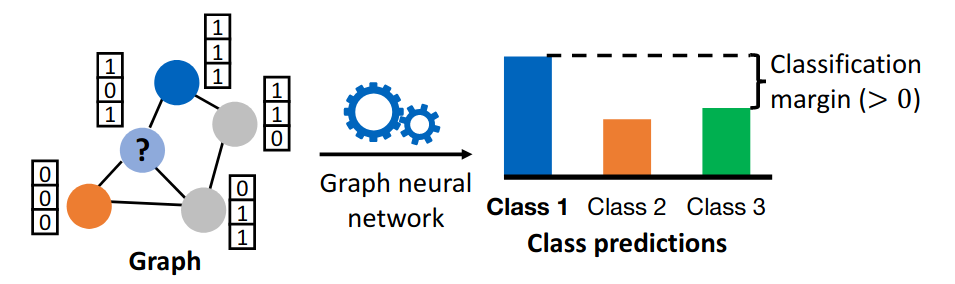
\includegraphics[width=0.5\textwidth]{img/before_pert.png}
    \caption{Classification margin before perturbation \cite{Zuegner_2019}}
    \label{fig:before_pert}
\end{figure}

Fig. \ref{fig:after_pert}, on the other hand, introduces two perturbations to the node attributes that lead to a negative
classification margin and therefore not to certifiable robustness.

\vfill
\pagebreak

\begin{figure}[h]
    \centering
    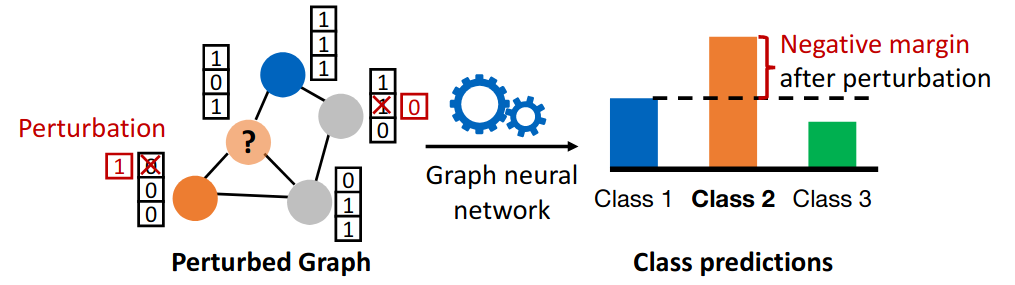
\includegraphics[width=0.5\textwidth]{img/after_pert.png}
    \caption{Classification margin after perturbation \cite{Zuegner_2019}}
    \label{fig:after_pert}
\end{figure}

To be able to solve the optimization problem in \ref{eq:1}, the authors have to find a way of treating the challenging
problems of a discrete data domain together with a nonconvex activation function in $f_{\theta}^t$. \cite{Zuegner_2019}
They tackle those issues by efficiently computing lower bounds on the minimum of the problem in \ref{eq:1} via relaxations 
of the GNN and the data domain. The idea is that a positive lower bound indicates the robustness of the classifier under 
the defined set of feasible perturbations.
To end up with a convex objective function in the optimization problem in \ref{eq:1}, a relaxation of the ReLU is required. \cite{Zuegner_2019} 
For such a relaxation, there are several methods published in the literature and the one, the authors follow,
leads to a linear objective function which determines a lower bound for the optimal value of the initial problem.
Although they end up with a linear problem (all constraints are linear as well), which can be solved with a specially optimized LP-solver,
a possibly huge set of variables in such a model that would reduce the efficiency, lets them consider a different approach.
Since every feasible solution of the dual problem provides a lower bound for the optimal solution of the primal problem, 
the dual of the LP is considered. \cite{Zuegner_2019} The authors summarize the idea as follows:
\begin{quote}
    \emph{"[...] if we find any dual-feasible solution for which the objective function of the dual is positive, we know that the minimum of 
    the primal problem has to be positive as well, guaranteeing robustness of the GNN w.r.t. any perturbation in the set."} \cite{Zuegner_2019}
\end{quote}

Since it is not necessary to obtain an optimal solution for the dual problem (it suffices to find a feasible solution), the robustness certificates
can be computed in a very efficient manner. As seen, the robustness of a node can be certified by positive dual values for each $y \neq y^{\ast}$.
In contrast, to provide certificates for non-robustness, one has to consider the primal values that have to be negative for one $y \neq y^*$. \cite{Zuegner_2019}
However, it is not guaranteed that each node falls into one of the two cases, which leaves certain nodes that can not be certified.
The authors highlight that reasonable (tight) upper and lower bounds are of great importance for robustness certification based on their method
and that those bounds can be used for backpropagation in the robust training procedure that will be presented in section \ref{subsec:robust_training}.\newline
The certification of robustness for trained GNNs is of course a very useful tool for practical applications, 
but, as the authors claim, the next step would be to achieve provable robustness of a model via training,
which will be considered in the following section.

\subsubsection{Robust Training}
\label{subsec:robust_training}

As seen in the previous section, the dual problem yields lower bounds on the classification margin
between the labels $y$ and $y^{\ast}$ for node $t$.
The authors define a $k$-dimensional vector $p_{\theta}^t$ that contains the solutions of the dual program
for a label $k$ compared to the label $y$. The node $t$ can be determined as being certifiably robust if $p_{\theta}^t < 0$
for all entries except the one for $y^{\ast}$, for which $y^{\ast} = 0$ holds. \cite{Zuegner_2019}
As a starting point for a training objective serves the following common objective function for classification tasks:
\begin{gather}
    \min_{\theta} \sum_{t \in \mathcal{V}_L} \mathcal{L} (f_{\theta}^t (\dot{X}, \dot{A}), y_t^{\ast})
\end{gather}
where $\mathcal{V}_L$ is the set of labeled nodes, $\mathcal{L}$ is the cross entropy function and $y_t^{\ast}$ represents
the label of node $t$ that is either given or predicted.
It is only a starting point, because they instead build on an objective from the literature that they call \textit{robust cross entropy loss},
which leads to an increased robustness of classical neural networks and provides an upper bound on the worst-case loss \cite{Zuegner_2019}:
\begin{gather}
\label{eq:between}
    \min_{\theta, \{\Omega^{t, k}\}_{t \in \mathcal{V}_L, 1 \leq k \leq K}} \sum_{t \in \mathcal{V}_L} \mathcal{L} (p_{\theta}^t (y_t^{\ast}, \Omega^{t, \cdot}), y_t^{\ast})
\end{gather}
To prevail the classical problem of overconfidence and to establish guaranteed robustness, the authors introduce 
a loss function that they call \textit{robust hinge loss}:
\begin{gather}
\label{eq:between_2}
    \mathcal{\hat{L}}_M (p, y^{\ast}) = \sum_{k \neq y^{\ast}} \max \{0, p_k + M\}
\end{gather}
The node $t$ is certifiably robust and guaranteed to have a margin $\geq M$ to the decision boundary if $\mathcal{\hat{L}}_M (p, y^{\ast}) = 0$
in equation \ref{eq:between_2}. \cite{Zuegner_2019}
In the final objective function in \ref{eq:2}, the authors merge their \textit{robust hinge loss} with the cross entropy function:
\begin{gather}
\label{eq:2}
    \min_{\theta, \Omega} \sum_{t \in \mathcal{V}_L} \mathcal{\hat{L}}_M (p_{\theta}^t (y_t^{\ast}, \Omega^{t, \cdot}), y_t^{\ast}) + \mathcal{L} (f_{\theta}^t (\dot{X}, \dot{A}), y_t^{\ast})
\end{gather}
The advantage compared to the \textit{robust cross entropy loss} is that the cross entropy function works with the exact
version of the GNN. \cite{Zuegner_2019}
Therefore, the authors only use the relaxed version to assure robustness while keeping with the exact version for node prediction.
In case every node is robust, $\mathcal{\hat{L}}_M = 0$ holds and the whole objective reduces to the simple cross entropy loss
on the original version of the GNN. \cite{Zuegner_2019}
So far, only the labeled nodes $\mathcal{V}_L$ are considered in \ref{eq:2}. To bridge the gap to the semi-supervised setting,
the authors also provide robustness guarantees for unlabeled nodes by extending the \textit{robust hinge loss} as depicted in \ref{eq:3}.
The objective in \ref{eq:3} is based on the idea of using the exact version of the network for classification while every node is guaranteed to have a margin
$\geq M$ from the decision boundary against every possible perturbation that is part of the defined attack model. \cite{Zuegner_2019}
The second margin $M_2$ is used for the unlabeled nodes $\mathcal{V} \backslash \mathcal{V}_L$.
\begin{multline}
\label{eq:3}
    \min_{\theta, \Omega} \sum_{t \in \mathcal{V}_L} \mathcal{\hat{L}}_{M_1} (p_{\theta}^t (y_t^{\ast}, \Omega^{t, \cdot}), y_t^{\ast}) + \mathcal{L} (f_{\theta}^t (\dot{X}, \dot{A}), y_t^{\ast}) \\
    + \sum_{t \in \mathcal{V} \backslash \mathcal{V}_L} \mathcal{\hat{L}}_{M_2} (p_{\theta}^t (\tilde{y}_t, \Omega^{t, \cdot}), \tilde{y}_t)
\end{multline}
The authors conclude that due to the differentiability of the dual program and the activation bounds,
the approach enables the training of a robust GNN using standard software.

\subsubsection{Experimental Evaluation and Conclusion}

The work (\cite{Zuegner_2019}) ends with an experimental evaluation of the approaches on the common data sets \textsc{Cora-ML}, 
\textsc{Citeseer}, and \textsc{PubMed}. First, the robustness of traditionally trained GNNs is evaluated using the presented
certification approach (cf. \ref{subsec:robustness_certification}) and afterwards, it is shown that the robust training procedure
(cf. \ref{subsec:robust_training}) significantly improves the robustness of GNNs without strong negative effects on the predictive accuracy.
As one would expect, the labeled set of nodes exhibits on average a higher robustness as the unlabeled one.
The following important observations are highlighted by the authors:
\begin{enumerate}
    \item Many of the provided certificates are tight.
    \item There is only a small fraction of nodes for which no certificate can be provided.
    \item Traditionally trained GNNs are only certifiably robust against negligible perturbations.
\end{enumerate}
Moreover, they analyze which properties are involved in making nodes robust or non-robust and identify neighborhood purity
as a key factor. 
They are observing a trade-off that says that many neighbors imply a large surface for potential attacks, while nodes 
with a lower degree are less stable and therefore stronger affected by individual neighboring attacks.
Regarding the robust training, they can show that their method significantly increases the number of robust nodes. 
If the perturbation budget for which the model was trained is considered, almost all the nodes are certifiably robust. \cite{Zuegner_2019}
Additionally increased is the general amount of certifiable nodes. There are even examples for nodes that have been certified as being
non-robust before, that become certifiably robust after the procedure.\newline

\textbf{Conclusion}\newline

The work presented in this section introduced the first methods for provable robustness of graph neural networks against
perturbations of node attributes. A major focus of the work was about being able to compute robustness certificates in an efficient
manner, which was achieved by several relaxations and a well justified consideration of dual feasible solutions instead of the optimal
solution values. Another fundamental result provided by Zügner et al. \cite{Zuegner_2019} is the fact that traditionally trained graph neural
networks are not robust and that the robust training procedure presented in the work is indeed able to significantly strengthen the robustness
of GNN models. The perhaps most important aspect is that the strengthened robustness does not have a significant negative effect on the predictive accuracy.
As future work, they already bridge to the next section which considers perturbations of the graph structure.

\subsection{Robustness Certification for Graph Structure Perturbations}
\label{sec:paper_three}

As announced in the previous section, the next step is to consider perturbations of the graph structure,
which means that the graph structure itself can be modified by an attacker.
In this section, the approaches of Zügner et al. \cite{10.1145/3394486.3403217} will be described, in which the
problem of certifiable robustness of GCNs against structural perturbations is tackled. 
Since these kind of perturbations attack, and thus modify, the message passing scheme, they are considered to be particularly challenging. \cite{10.1145/3394486.3403217} 
The authors reformulate the problem as a jointly-constrained bilinear program and develop a branch-and-bound procedure 
to provide lower bounds on the optimal solution value. The attack model that is used in the work is based on the idea that an attacker 
is able to insert new edges to the graph. Such a scenario could for example occur in web-based applications where edges represent friends, 
likes or follows in social media. \cite{10.1145/3394486.3403217}
The high-level idea, which is visualized in fig. \ref{fig:high_level}, is that there is a clean graph that is reachable by removing
these adversaries that could have changed the model's prediction.
The authors summarize the idea of their certificates as follows:
\begin{quote}
    \emph{"A certificate issued by our method states that a node's prediction could not have been altered by edges potentially
    inserted by an attacker."} \cite{10.1145/3394486.3403217}
\end{quote}

\begin{figure}[h]
    \centering
    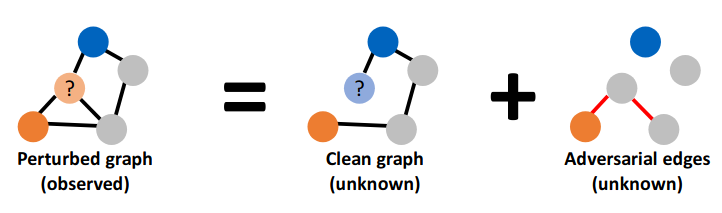
\includegraphics[width=0.5\textwidth]{img/high_level_graph_pert.png}
    \caption{High-level idea of Zügner et al. \cite{10.1145/3394486.3403217}}
    \label{fig:high_level}
\end{figure}

\vfill
\pagebreak

There are three major challenges identified in the work:

\begin{figure}[h]
    \centering
    \begin{enumerate}
        \item The search for optimal perturbations is not efficient due to the general nonconvexity of neural networks.
        \item Enumerating the set of feasible perturbations is of course not efficiently possible as well, because the cardinality of the
        set is growing exponentially with the perturbation budget.
        \item In contrast to the certificates of the approach in section \ref{sec:paper_two}, here the changed structure could change 
        the propagation of embeddings.
    \end{enumerate}
    \caption{Major challenges to be solved.}
    \label{fig:challenges}
\end{figure}

The first challenge is also a problem for traditional neural networks and the approach already used
in section \ref{sec:paper_two}, which relaxes the ReLU activation function, is applied again. \cite{10.1145/3394486.3403217}
For the second challenge, the authors can not recycle another approach, but have to come up with new solutions.
They show that a continuous relaxation, as used for the binary attributed data in section \ref{sec:paper_two}, 
is not applicable for attacks on the graph structure and instead work directly on the degree-normalized message passing matrix 
of the GCN which already consists of continuous values.
Another unstudied question is posed by the third challenge that requires a way to handle a modified structure (message passing scheme). \cite{10.1145/3394486.3403217}
The authors see the problem in the fact that the message passing scheme, i.e. the matrix, in contrast to the input features considered
in section \ref{sec:paper_two}, are used in every layer of the network and not only in the input layer.
That causes nonconvex constraints after the ReLU relaxations. \cite{10.1145/3394486.3403217}
As mentioned, the authors reformulate the problem as a jointly-constrained bilinear program and develop a branch-and-bound procedure 
to provide lower bounds on the optimal solution value.
The lower bounds can be seen as worst-case change for the prediction of a node and are therefore used as 
robustness certificates where a positive value indicates that the prediction of a node will not
change when being exposed to a feasible attack . \cite{10.1145/3394486.3403217}

\subsubsection{Robustness Certification Technique}

The problem is outlined as a semi-supervised node classification task in a graph $G = (A, X)$ with $D-$dimensional node attributes
where $A \in \{0, 1\}^{N \times N}$ is the adjacency matrix and $X \in \mathbb{R}^{N \times D}$ are the attributes of the nodes.
Just as in section \ref{sec:paper_two}, $V_L \subseteq V$ is the subset of labeled nodes with labels $C = \{1, 2, ..., K\}$.
Also as in the previous section, $\theta$ summarizes the trainable weights of the GNN that can be learned using the labeled nodes $V_L$
by minimizing the cross entropy loss. \cite{10.1145/3394486.3403217}
The message passing matrix that defines how activations are propagated through the GNN can be obtained
by a defined transformation $\mathcal{T}(A)$ to the adjacency matrix. \cite{10.1145/3394486.3403217}
As always in classification tasks, the aim is to assign labels to the nodes.
The network's output $H_{vc}^{(L)}$ is the probability of assigning label $c$ to node $v$. \cite{10.1145/3394486.3403217}\newline
At first, the authors define the optimization problem that is to be solved.
The starting point is an already trained GNN with weights $\theta$. The input graph that is represented by the adjacency matrix $A$
may already be perturbed. At this point, the main idea, visualized in fig. \ref{fig:high_level}, comes into play, which is that
the graph represented by $A$ can be reached from the \textquote{clean} unperturbed version of the graph represented by an adjacency 
matrix $A^{\ast}$ by a set of feasible perturbations against the graph structure, e.g. adversarial edges. \cite{10.1145/3394486.3403217}

\vfill
\pagebreak

The authors guarantee the robustness for a single node at a time, i.e. they assure that the specific node under 
consideration is not changing its prediction after a feasible attack.
The worst-case margin between $y^{\ast}$ and $y$ is computed as the following optimization problem where $y^{\ast}$ defines the given / predicted 
label of node $t$ and $\mathcal{A}(A)$ defines the set of feasible perturbations.
\begin{gather}
\label{eq:4}
    m^t (y^{\ast}, y) := \min_{\tilde{A}} f_{\theta}^t (X, \mathcal{T}(\tilde{A}))_{y^{\ast}}
    - f_{\theta}^t (X, \mathcal{T}(\tilde{A}))_y \\
    s.t. \tilde{A} \in \mathcal{A}(A) \nonumber
\end{gather}
The GNN is claimed to be robust under the set of feasible attacks for the node $t$ in question,
if $m^t (y^{\ast}, y) > 0 \thinspace \forall \thinspace y \neq y^{\ast}$.
Therefore, just as for the optimization problem in section \ref{sec:paper_two}, if the minimum in \ref{eq:4} is positive, 
there is no feasible perturbation to the graph structure that would cause a prediction change of node $t$. \cite{10.1145/3394486.3403217}\newline
Now we get back to the previously mentioned challenges (cf. \ref{fig:challenges}) that prevent an easy and efficient optimization 
of the problem in \ref{eq:4}.
The authors are able to bypass the hard, or inefficient part of the problem by again computing lower bounds instead of optimal values.
More precisely, they perform the following three steps to compute lower bounds on the original problem that
allow to answer the question of robustness:
\begin{itemize}
    \item Replace the binary adjacency matrix $A$ by the continuous message-passing-matrix $\mathcal{T}(A)$.
    \item Relax the activation function of the GNN.
    \item Rephrase the problem as jointly-constrained bilinear program and solve it with branch-and-bound.
\end{itemize}
A positive lower bound indicates robustness under the defined attack model. \cite{10.1145/3394486.3403217}\newline

\textbf{Optimization over the graph structure}\newline

In order to be able to cope with the second challenge mentioned in fig. \ref{fig:challenges}, the set of feasible perturbations
is restricted in such a way that on the one hand the sheer size of the set is limited and on the other hand
it reflects perturbations that could actually occur in practical applications. \cite{10.1145/3394486.3403217}
The authors again use the $L_0$ norm, in this case to measure the number of perturbed elements in $A$.
To do that, they transfer the idea of local and global $L_0$ constraints on the node attributes used in the previous paper 
discussed in section \ref{sec:paper_two} to structural perturbations, which means that there are allowed to be at most
$q_i \in \mathbb{N}$ local adversarial edges to a specific node $i$ and at most $Q \in \mathbb{N}$ global adversarial
edges inserted into the whole graph. \cite{10.1145/3394486.3403217}
This approach refers to the high-level idea visualized in fig. \ref{fig:high_level}, i.e. that the perturbed graph structure
differs from the original (clean) structure by a certain set of inserted adversarial edges.\newline
Continuous relaxation would be the common way of dealing with intractable discrete optimization problems,
but in this case, due to the minimization over $\tilde{A}$ in the objective function, this is not an option. \cite{10.1145/3394486.3403217}
Instead, the authors propose to use the degree normalized message-passing-matrix $\hat{A}$ in its continuous nature.
As a result, the optimization problem in \ref{eq:4} is replaced by the following problem, which not only avoids 
the intractable optimization over a discrete variable, but also the nonconvex degree normalization process
since the message-passing-matrix $\hat{A}$ is now directly passed to $f_{\theta}^t$ as input. \cite{10.1145/3394486.3403217}
\begin{gather}
\label{eq:5}
    \hat{m}^t (y^{\ast}, y) := \min_{\hat{A}} f_{\theta}^t (X, \hat{A})_y^{\ast}
    - f_{\theta}^t (X, \hat{A})_y \\
    s.t. \hat{A} \in \mathcal{\hat{A}}(A) \nonumber
\end{gather}

\vfill
\pagebreak

It is crucial to define the set $\mathcal{\hat{A}}(A)$ of possible message passing matrices in a way that it contains
every possible matrix that could result from first performing discrete perturbations to $A$ and afterwards 
degree-normalizing the resulting binary matrix $\tilde{A}$, only then it holds that $\hat{m}^t (y^{\ast}, y) \leq m^t (y^{\ast}, y)$, 
i.e. the result of \ref{eq:5} provides a lower bound on the optimal solution of the optimization problem in \ref{eq:4}. \cite{10.1145/3394486.3403217}
The authors are able to derive constraints to generate message passing matrices $\mathcal{\hat{A}}$
that are valid, tight, and convex to enable efficient optimization.
Finally, a positive value of \ref{eq:5} indicates a certificate. \cite{10.1145/3394486.3403217} \newline

\textbf{Relaxation of the neural network}\newline

As stated in the first challenge in fig. \ref{fig:challenges}, the objective function of the GNN is hard due to the non-convexity.
Therefore, the authors again apply a relaxation approach from their previous paper \cite{Zuegner_2019}, which causes the output $H$ 
of the ReLU activation function to no longer be deterministic, but considered to be a variable and combine it with ideas
of another approach from the literature.\newline

\textbf{Jointly constrained bilinear program}\newline

Combining the relaxed GNN with the constraints on the message-passing-matrix, the objective function in \ref{eq:5} 
can be reformulated as a bilinear objective function. \cite{10.1145/3394486.3403217}
Afterwards, they add another artificial constraint that does not change the solution, but enables them to use 
a principle proposed in the literature which allows them to solve the jointly constrained bilinear optimization problem.
The convex envelope of the objective function is used to compute lower bounds and additionally, a branch-and-bound procedure is used
to recursively divide the problem into sub-problems. In each iteration, the upper and lower bounds become more and more precise
and the idea is to stop as soon as possible. It is important to note that it is not necessary to find the optimal solution of 
the bilinear problem, only its sign is of relevance. \cite{10.1145/3394486.3403217}
Consequently, there are two possible outcomes: A positive lower bound indicates successfully certified robustness, while a negative
lower bound only states that no robustness certificate can be given and not non-robustness. \cite{10.1145/3394486.3403217}\newline

\subsubsection{Experimental Evaluation and Conclusion}

As in the previous paper presented in section \ref{sec:paper_two}, an experimental evaluation of the approaches on the benchmark data sets 
\textsc{Cora-ML}, \textsc{Citeseer}, and \textsc{PubMed}. is provided.
The authors evaluate the proposed robustness certification technique against attacks on the graph structure
based on three different local $q$ and global $Q$ perturbation budgets with which they perform gradient-based attacks.
This approach enables them to estimate the number of non-robust nodes, although the computation of the precise number would be intractable. \cite{10.1145/3394486.3403217}
As one would expect, higher perturbation budgets cause fewer nodes that can be considered as being certifiably robust and 
more non-robust nodes. \cite{10.1145/3394486.3403217}
Another hint to the general non-robustness of GCN models is given by the fact that it suffices to remove one edge from the graph
to cause predictive changes in a significant portion of the nodes. \cite{10.1145/3394486.3403217}
A further crucial observation is that 'classical' adversarial training procedures based on the idea of adding adversarially
perturbed examples to the training data, such as the perturbed graph in fig. \ref{fig:high_level}, are not leading to a higher robustness
of the model \cite{10.1145/3394486.3403217}, which confirms the relevance of the work.
Only the training for robustness against perturbations of the node attributes that is considered in section \ref{sec:paper_two} is able to do so.\newline

In summary, the authors introduce first approaches for certifiable robustness against structural perturbations for graph convolutional networks.
The main idea is to reformulate the problem as a jointly constrained bilinear program and to efficiently solve that using a branch-and-bound
method. The branch-and-bound method recursively divides the problem into linear sub-problems that can be solved by specially optimized LP-solvers (e.g. CPLEX).
For a large fraction of the nodes, the authors are able to provide a clear decision of robustness / non-robustness.
Overall, the presented work provides a very efficient way of robustness certification.

\subsection{Robustness guarantee of arbitrary GNNs for node and graph classification}
\label{sec:paper_four}

The latest work on certifiable robustness of GNNs against adversarial perturbations is provided by Wang et al. \cite{Wang_2020}
who consider robustness guarantees for arbitrary graph neural network models. The studied task is again a classification task,
but this time classification on the node- as well as on the graph-level.
Like the approaches of Zügner et al. \cite{10.1145/3394486.3403217} and Bojchevski et al. \cite{bojchevski2019certifiable},
they address certifiable robustness of GNNs against perturbations of the graph structure. 
In contrast to to the previous papers described in section \ref{sec:paper_two}
and \ref{sec:paper_three}, which deal with specific GNN models, they provide robustness guarantees for arbitrary GNNs.
To achieve that, they make use of an extended version of the \textit{randomized smoothing} method, which essentially adds noise 
to the elements of the training data set in order to establish robustness. \cite{Wang_2020}
The authors extend the basic \textit{randomized smoothing} such that they are able to handle non-continuous data structures, i.e. graphs.
A certain \textit{certified perturbation size} $K$ is defined with the intention of setting a limit onto the number of adversarial edge additions
or removals such that a GNN is considered to be robust if there is no change of prediction when the number of perturbations is $\leq K$. \cite{Wang_2020}\newline

To summarize, they extend the \textit{randomized smoothing} approach to discrete (binary) data structures such as graphs 
and thereby enable robustness certification for arbitrary graph neural networks against structural perturbations.
Finally, they evaluate their approach on various benchmark instances for node and graph classification tasks.

\section{Conclusion}
\label{sec:conclusion}

In this paper, a concise overview of the current state of research in the domain of graph (convolutional) neural networks with a focus on the robustness 
of the models was provided. As seen throughout the sections, GNNs can be applied very successfully to a wide range of practical tasks.
What has prevented its frequent use in practice so far is the fact that GNNs are not at all robust against adversarial perturbations of the graph structure
and the node attributes, which has been proven by numerous publications discussed in section \ref{sec:literature}.
As long as it is possible that small changes to the input data cause entirely different results, it is not reasonable to
apply the models in any kind of safety-critical application or in areas where legal certainty must prevail.\newline
Three main lines of research in the domain of robust GNNs have been identified in this work. In the first phase, it was shown that GNNs are prone to adversarial attacks.
The second phase introduced defense mechanisms against such attacks or training procedures to strengthen the robustness. However, these approaches
are generally just providing mitigations for certain scenarios and not guaranteeing robustness in any case.
The third phase, which was the main consideration of this work, discussed in section \ref{sec:main_section}, only recently started to tackle this problem. 
Approaches appeared that are able to not only provide mitigations to adversarial attacks in some scenarios, but to give provable guarantees about 
the (non-)robustness of a GNN with regard to an attack model, which is crucial to use them in real-world applications.\newline
Although this phase only started recently, there have already been quite effective approaches for certified robustness presented in section \ref{sec:main_section}.
Nevertheless, there is of course a lot of room for improvement and generalization.
Zügner et al. \cite{10.1145/3394486.3403217} for example suggest that it might be worthwhile to study training methods in which 
robustness is explicitly treated as the goal to be achieved.
Another promising future prospect is given by Wang et al. \cite{Wang_2020} who suggest to extend their method briefly described in 
section \ref{sec:paper_four} to not only certify robustness of GNNs against structural perturbations, but to also include perturbations
of the node attributes.
In addition, they plan to optimize the method by including and exploiting certain information about a GNN during the process.
On a less concrete level, it would also be interesting to find out what makes perturbations harmful and therefore
truly develop an understanding of the fundamental structure of the problem.
The approach of Jin et al. \cite{Jin_2020_Graph} goes in this direction in a way, although they are not considering certifiable robustness.
Their work is rather belonging to the second phase, dealing with mitigations, as the proposed framework
\textit{Pro-GNN} enables a reasonable defense method in some scenarios.
Nonetheless, they highlight an important observation which is that graph structures representing problems from the real-world often
share some intrinsic properties that are likely to be violated by adversarially perturbed graphs.
Eventually, the approaches of the third phase outlined in this work assume a certain attack model under which robustness guarantees are provided.
If a general understanding of the underlying mechanisms of harmful perturbations can be established, there could be even more room
for generalizations of attack models to guarantee robustness for.

\vfill
\pagebreak

\bibliographystyle{acm}
\bibliography{bibliography}

\end{document}